\section{Pre-training: RES task performance}
\label{sec:res-task}
In the first phase (Section \ref{res-task}), I train two equivariant GNN models on the RES task, using the ATOM3D dataset. The ATOM3D RES \cite{atom-3d} dataset is large, with over 3 million graph samples. As a consequence, the models have taken around a week each to train using one NVIDIA A100 GPU. Due to this constraint, I report the test accuracy resulting from a single training run on each of the two models. 

Table \ref{model-accuracy} summaries the test accuracies of the trained models.
\begin{table}
\caption{Classification accuracies on the ATOM3D RES dataset.}
\label{model-accuracy}
\vskip 0.15in
\begin{center}
\begin{small}
\begin{sc}
\begin{tabular}{@{}lcc@{}}
\toprule
Model & \begin{tabular}[c]{@{}c@{}}Reported test accuracy\end{tabular} & \begin{tabular}[c]{@{}c@{}}My test accuracy\end{tabular} \\ \midrule
EQGAT & 0.540                                                             & 0.524                                                        \\
GVP   & 0.527                                                             & \textbf{0.580}                                               \\ \bottomrule
\end{tabular}
\end{sc}
\end{small}
\end{center}
\vskip -0.1in
\end{table}
I was unable to replicate the test accuracy reported by \citet{eqgat2} on the RES task. One possible reason is a mismatch in the hyperparameter configuration, which the original authors do not report for the RES task. However, due to the computational constraints mentioned above, it was unfeasible to perform further hyperparameter tuning to determine the best setup. 

Surprisingly, I report a much higher accuracy for the GVP architecture than originally stated in \cite{gvp2}. One possible explanation is that \citet{gvp2} train their GVP model on 1 million sampled graphs from the ATOM3D RES dataset, therefore using only a third of the full training dataset. In light of this, I report that the GVP model trained on the full ATOM3D RES dataset achieves a new state-of-the-art performance on the RES task, with an accuracy of \textbf{58\%}. 

\subsection{How good should a model be?}
\label{training-discussion}
Since I use these models as mutation generation engines, one tricky question is when to stop training: that is, when the model predicts an amino acid wrongly, is it because the model made a mistake, \textit{or is it because Nature made a mistake?} In this project, I stop training after 40 epochs due to computational constraints, although the validation curves of both models do not show clear signs of overfitting, as can be seen in Figure \ref{train-plots}.

\begin{figure}[!htb]
    \centering
    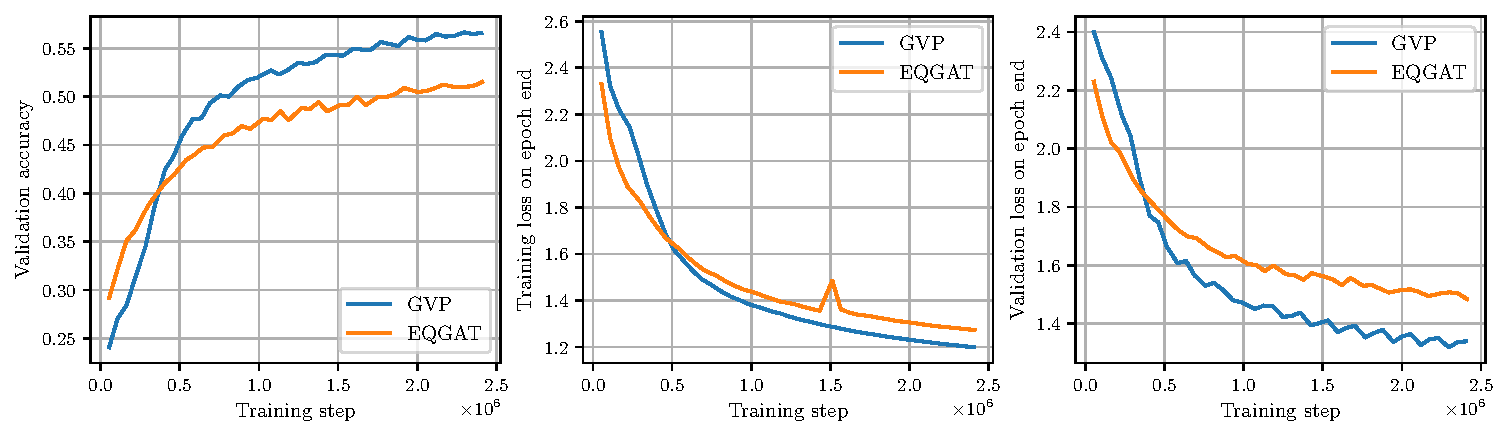
\includegraphics[width=\textwidth]{masters-report/figures/validation_acc.pdf}
    \caption{Accuracy and loss values across 40 epochs.}
    \label{train-plots}
\end{figure}

As it is discussed in Section \ref{mutation-discard}, I perform an ablation study in which I compare the performance of the two ranking techniques when I ignore mutations at positions that the models got wrong. Since the models perform \textit{better} when I discard these mutations, this is an indication that the models themselves are still \textit{undertrained}, thereby having a higher capacity for mutation generation than the one achieved in this project. 

\section{Evaluation metrics}
The main aim of my approach to mutation generation is to find mutations that are better than the wildtype sequence. To quantify how good my models are for predicting promising mutations, I am particularly interested in 3 metrics: Spearman's rank correlation for better than wildtype mutations, the top 10 precision, and the top 10 recall. I briefly present the motivation behind all three metrics below. 

\subsection{Spearman's rank correlation} 
The Spearman rank correlation, also known as Spearman's $\rho$, is a statistical measure that assesses the strength and direction of the monotonic relationship between two variables. It is formally defined as the Pearson correlation coefficient between rank variables. For a sample of size $n$, the $n$ raw scores $X_i$ and $Y_i$ are converted to ranks $R(X_i)$ and $R(Y_i)$. Then, the coefficient $r_s$ is computed as:
\begin{equation}
    r_s = \frac{\text{cov}(R(X), R(Y))}{\sigma_{R(X)}\sigma_{R(Y)}}
\end{equation}
where $\sigma_{R(X)}$ and $\sigma_{R(Y)}$ are the standard deviations of the rank variables. 

I am interested in quantifying the performance of my approach in predicting single-point mutations that are better than the wildtype sequence. Hence, one of the metrics I am interested in is the Spearman rank correlation for better than wildtype mutations only. That is, I discard predicted mutations for which the true fitness (found in the ProteinGym dataset) is lower than the fitness of the wildtype sequence.

In contrast to this approach, \citet{tranception}, who propose Tranception, only report the \textit{average} Spearman rank correlation between their model's prediction and the true fitness. To produce a fair comparison, I report both the average Spearman and the better than wildtype Spearman for the EQGAT and GVP, as well as for representatives of the sequence-based approaches: Tranception \cite{tranception}, ESM-1v \cite{meier2021language}, and the MSA Transformer \cite{Rao2020}.

\subsection{Precision and recall} 

Precision and recall are two metrics used in evaluating the performance of classification models, particularly in the field of information retrieval and machine learning. They are commonly used together to provide a comprehensive assessment of a model's effectiveness.

% Precision measures the proportion of correctly predicted positive instances out of all instances predicted as positive. It focuses on the reliability of positive predictions, hence a high precision means that the model has a low rate of false positives. The formula for precision is:
% \begin{equation}
% \text{Precision} = \frac{\text{True Positives}}{\text{(True Positives + False Positives)}}
% \end{equation}
% Recall can be considered complimentary to precision, as it measures the proportion of correctly predicted positive instances out of all actual positive instances. It focuses on the overall ability of the model to identify positive instances. The formula for recall is:
% \begin{equation}
% \text{Recall} = \frac{\text{True Positives}}{\text{(True Positives + False Negatives)}}
% \end{equation}
% As mentioned before, we are interested in the models' ability to predict promising mutations. We therefore treat mutations as positives if they are better than the wildtype and negatives otherwise. 

\paragraph{Top-k precision and recall.}
Top-k precision measures the proportion of correctly predicted positive instances among the top-k predictions made by the model.
The formula for top-k precision is:
\begin{equation}
\text{Top-k Precision} = \frac{\text{(Number of true positives within top-k)}}{k}
\end{equation}
Top-k recall measures the proportion of correctly predicted positive instances among all the relevant instances, considering only the top-k predictions made by the model. The formula is:
\begin{equation}
    \text{Top-k Recall} = \frac{\text{(Number of true positives within top-k)}}{\text{(Total number of better than wildtype mutations)}}
\end{equation}

Note that the recall is calculated relative to the number of mutations predicted by each model, rather that relative to the total number of mutations in each DMS assay from ProteinGym. 

In this project I report the top-10 precision and the top-10 recall, because my aim is to build an easy to use tool for researchers to accelerate their discovery process, and having a list of the top 10 mutations that are considered promising is a straightforward way of aiding the exploratory process. 

\section{Mutation generation}
\label{sec:mutation-generation-results}
For mutation ranking, I use the DMS assays of 49 sequences out of the total of 87 that exist in the ProteinGym substitutions dataset. These 49 sequences are either monomers or homo-oligomers for which I could find either a complete experimental structure or an AlphaFold predicted structure, as discussed in Section \ref{sec:structure-recovery}.

Before presenting the results to mutation ranking, it is important to note that my approach generates mutations, rather than predicting the fitness of already existing ones. This means some of the proposed mutations will not exist in the ProteinGym dataset; when this is the case, I discard them, as there is no other way of evaluating their fitness other than in the wet lab, and this would be beyond the scope of this project.

Additionally, when ranking the mutations generated by the EQGAT and the GVP models, I choose to \textit{discard} mutations proposed at positions where the models failed to predict the true wildtype residue. Formally, given a sequence $x_1x_2\dots x_n$, I discard all mutations $\mathbf{m}_i^a$ proposed for position $i$ if there exists an amino acid $b$ such that $S(i, b) > S(i, x_i)$. A broader discussion on the motivation behind this design choice can be found in Section \ref{mutation-discard}. 

Table \ref{mutation-generation} summaries the performance of my approach to mutation ranking. As we can see, although the MSA Transformer \cite{tranception} achieves the highest overall Spearman rank correlation, it performs poorly when only considering mutations that are better than the wildtype. 
A per-dataset breakdown of the performance of EQGAT, GVP, and Tranception can be found in Appendix \ref{appendix:per-dataset-breakdown}.

\begin{table*}[!htb]
\caption{\raggedright{Ranking performance of the models across 49 DMS assays. Numbers in \textbf{bold} represent the highest score per column, while numbers with an \underline{underline} represent the second highest score per column. We note that two equivariant GNNs have the highest rank correlation for better than wildtype mutations.}}
\label{generation-results}
% \vskip 0.15in
\begin{center}
\begin{small}
\begin{sc}
\begin{tabular}{@{}ccccccc@{}}
\toprule
\multirow{2}{*}{Model} & \multirow{2}{*}{\begin{tabular}[c]{@{}c@{}}Ranking \\ strategy\end{tabular}} & \multirow{2}{*}{\begin{tabular}[c]{@{}c@{}}Top 10\\ precision\end{tabular}} & \multirow{2}{*}{\begin{tabular}[c]{@{}c@{}}Top 10\\ recall\end{tabular}} & \multicolumn{3}{c}{Spearman's rank correlation}                                                                                       \\ \cmidrule(l){5-7} 
                       &                                                                              &                                                                             &                                                                          & All        & \begin{tabular}[c]{@{}c@{}}Worse than \\ WT\end{tabular} & \begin{tabular}[c]{@{}c@{}}Better than \\ WT\end{tabular} \\ \midrule
EQGAT                  & Positional                                                                   & 0.486                                                                       & \underline{0.187}                                                              & 0.223          & 0.128                                                    & 0.118                                                     \\
EQGAT                  & Global                                                                       & 0.491                                                                       & 0.072                                                                    & 0.262          & 0.154                                                    & \underline{0.157}                                               \\
GVP                    & Positional                                                                   & 0.462                                                                       & \textbf{0.419}                                                           & 0.106          & -0.009                                                   & \textbf{0.276}                                            \\
GVP                    & Global                                                                       & 0.426                                                                       & 0.100                                                                    & 0.202          & 0.128                                                    & -0.011                                                    \\ \midrule
Tranception            &                                                                              & \underline{0.619}                                                                 & 0.012                                                                    & \underline{0.429}    & \underline{0.299}                                              & 0.143                                                     \\
ESM-v1                 &                                                                              & 0.618                                                                       & 0.018                                                                    & 0.407          & 0.288                                                    & 0.135                                                     \\
MSA Trans.        &                                                                              & \textbf{0.638}                                                              & 0.018                                                                    & \textbf{0.434} & \textbf{0.327}                                           & 0.135                                                     \\ \bottomrule
\end{tabular}
\end{sc}
\end{small}
\end{center}
\vskip -0.1in
\end{table*}



\paragraph{The ranking approach.}
I note that the GVP model achieves the best ``better than WT'' Spearman rank correlation to the ProteinGym fitness values. This performance seems to be highly dependent on the type of ranking used, as the correlation drops from $\mathbf{0.27}$ to virtually $\mathbf{0}$ when switching from positional to global ranking. Additionally, positional ranking keeps only the \textit{top 3} mutations per position, hence this approach would actually generate \textbf{fewer} mutations instead of proposing worse ones. 
% This is also indicated by the high top-10 recall of the same approach, namely $\mathbf{0.41}$, which suggests that, on average, the top 10 mutations proposed by the GVP account for almost half of all the better than wildtype mutations the model generates (and are found in the ProteinGym dataset).

\paragraph{Data efficiency.}
EGNN models require a significantly smaller number of protein structures during training in order to reach a similar ranking correlation coefficient to the sequence-based models for mutations that are better than the wildtype. While these models are typically trained on massive amounts of data (e.g. 350 million sequences in the case of Tranception) my models are trained on fewer than 22k molecules from which local environments are sampled. This, coupled with the fact that these structural models have not reached their capacity (as mentioned Section \ref{training-discussion}), indicates that these EGNN models to be \textit{further fine-tuned} by small research groups for task specific purposes. 

\paragraph{Correlation to sequence-based models.}
As part of my analysis, I also compute the correlation between the better than wildtype predictions made by the EGNN models and Tranception. Per-model and per-dataset statistics can be found in \ref{tranception-correlation}; I note that the highest rank correlation I find is \textbf{0.212}, in the case of the EQGAT model. Since these approaches seem to be weakly correlated, I believe there are improvements to be gained from ensembling both structure- and sequence-based approaches.

Note that in the case of the EQGAT model, changing the ranking strategy does not result in a significant performance drop, indicating that the model identifies both the good positions and the good amino acids to perform mutations, but performs worse overall.

\subsection{Ablation studies}
The development of performant structure-based models for mutation generation involved design decisions that impacted how proteins are processed by my models and whether certain mutations are kept or discarded from the overall ranking. 
For the purposes of aiding future the engineering efforts of designing good structure-based methods, I report a few ablation studies that justify the decisions made for the main evaluation. A summary of the findings suggest the following: 
\begin{itemize}
    \item Discarding positions where the models cannot correctly identify the true wildtype amino acid increases the quality the mutation ranking (Tables \ref{ablation-correct-only-global} and \ref{ablation-correct-only-positional});
    \item Using the AlphaFold structure is \textit{not} detrimental to the generation of better than wildtype mutations (see Appendix \ref{appendix-exp-vs-alphafold}: Tables \ref{ablation-alphafold-global} and \ref{ablation-alphafold-positional});
    \item The EQGAT model works best with the full molecular structure, while the GVP model works best with the local environment (see Appendix \ref{appendix-full-vs-local}: Tables \ref{ablation-local-environment-global} and \ref{ablation-local-environment-positional}).
\end{itemize}

\subsubsection{Discarding wrongly predicted positions}
\label{mutation-discard}
As mentioned at the beginning of Section \ref{sec:mutation-generation-results}, I add an additional filter to my ranking techniques in order to increase the quality of the mutations proposed by the models. More specifically, I discard all mutations at a position that was classified incorrectly by the EGNN. An incorrect classification of a residue may indicate that the models do not have a good understanding of the biophysical properties of the residue's local environment. This is particularly damaging to the generation of meaningful mutations if a models assigns similarly low confidences to all 20 amino acids that are candidate for a position because it resorts to random guessing. 

I provide an ablation study to back up this design choice. Tables \ref{ablation-correct-only-global} and \ref{ablation-correct-only-positional} show how, overall, keeping all mutations generated by any structure-based model decreases its performance. 

\begin{table}[!hbt]
\caption{Model performance when performing \textbf{global} ranking using both wrongly and correctly predicted positions. Statistics averaged across for 49 DMS assays.}
\label{ablation-correct-only-global}
\vskip 0.15in
\begin{center}
\begin{small}
\begin{sc}
\begin{tabular}{@{}ccccc@{}}
\toprule
\multirow{2}{*}{Model} & \multirow{2}{*}{Positions used} & \multicolumn{3}{c}{Spearman's rank correlation}  \\ \cmidrule(l){3-5} 
                       &                                 & Average        & Worse than WT  & Better than WT \\ \midrule
EQGAT                  & all                             & 0.20           & 0.153          & 0.069          \\
EQGAT                  & correct only                    & \textbf{0.262} & \textbf{0.154} & \textbf{0.157} \\ \midrule
GVP                    & all                             & 0.093          & 0.076          & \textbf{0.014} \\
GVP                    & correct only                    & \textbf{0.202} & \textbf{0.128} & -0.011         \\ \midrule
Tranception            &                                 & 0.429          & 0.299          & 0.143          \\ \bottomrule
\end{tabular}
\end{sc}
\end{small}
\end{center}
\vskip -0.1in
\end{table}

\begin{table}[!hbt]
\caption{Model performance when performing \textbf{positional} ranking using both wrongly and correctly predicted positions. Statistics averaged across for 49 DMS assays.}
\label{ablation-correct-only-positional}
\vskip 0.15in
\begin{center}
\begin{small}
\begin{sc}
\begin{tabular}{@{}ccccc@{}}
\toprule
\multirow{2}{*}{Model} & \multirow{2}{*}{Positions used} & \multicolumn{3}{c}{Spearman's rank correlation}             \\ \cmidrule(l){3-5} 
                       &                                 & Average        & Worse than WT & Better than WT \\ \midrule
EQGAT                  & all                             & 0.124          & 0.100               & 0.061                \\
EQGAT                  & correct only                    & \textbf{0.223} & \textbf{0.128}      & \textbf{0.118}       \\ \midrule
GVP                    & all                             & 0.083          & \textbf{0.076}      & -0.018               \\
GVP                    & correct only                    & \textbf{0.106} & -0.009              & \textbf{0.276}       \\ \midrule
Tranception            &                                 & 0.429          & 0.299               & 0.143                \\ \bottomrule
\end{tabular}
\end{sc}
\end{small}
\end{center}
\vskip -0.1in
\end{table}

\paragraph{Analysing undertraining.}
We can get a better idea of the types of information that is learned by the EGNN models by looking at the confusion matrices between the true labels and the predicted labels in the ATOM3D RES test dataset, illustrated in Figure \ref{fig:confusions}. I compare these two matrices to the BLOSUM62 matrix, a scoring matrix commonly used in bioinformatics for sequence alignment; each cell represents the score for substituting one amino acid with another. Higher scores indicate a higher degree of conservation or similarity between the substituted amino acids.

I expect that models with meaningful inferred knowledge about the biophysical properties of amino acids to have a similar confusion matrix to the BLOSUM62 matrix; while some parts of the confusion matrix do resemble BLOSUM62 (e.g., Cystine (C) is not easily confused with any of its neighbouring amino acids), it seems that the models are still undertrained. I do, however, notice that the confusion matrices of the EQGAT and the GVP look similar to each other, indicating that they must be learning the same features from the training dataset.  

\begin{figure}
    \centering
    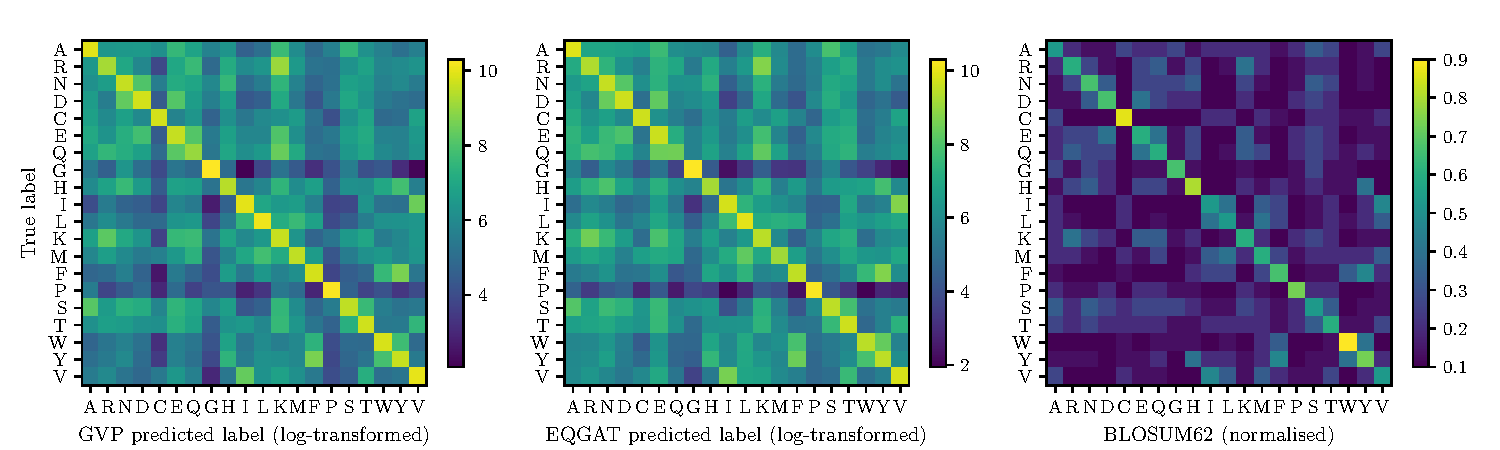
\includegraphics[width=\textwidth]{masters-report/figures/confusion_matrices.pdf}
    \caption{Comparison between the confusion matrices of EQGAT and GVP to the BLOSUM62 matrix.}
    \label{fig:confusions}
\end{figure}


% \subsubsection{Experimental structure vs. AlphaFold structures}


% As mentioned in Section \ref{sec:structure-recovery}, we expect the usage of AlphaFold structures to be detrimental to the overall performance of our models. To check whether this is indeed the case, we perform on ablation study on 14 of the 49 sequences we use in this project. These sequences have both a complete experimental structure and an AlphaFold structure, so we can compare the performance of our models using either one or the other. Since the ablation study presented in Section \ref{mutation-discard} makes it clear that mutations at wrongly predicted positions are detrimental to our models, we perform this second ablation study by also discarding mutations for positions that models get wrong.

% As presented in Tables \ref{ablation-alphafold-global} and \ref{ablation-alphafold-positional}, we find that there isn't a clear relation between using the AlphaFold structure and a decrease in the better than wildtype Spearman correlation, as it seeems to depend on both the model and the ranking strategy used. However, we notice notice that in 3 out of 4 cases, models rank \textit{worse than wildtype} mutations better when using the AlphaFold structure. 

% \begin{table}[!h]
% \caption{Model performance when performing \textbf{global} ranking using either AlphaFold or experimental features. Statistics are averages across 14 sequences.}
% \label{ablation-alphafold-global}
% \vskip 0.15in
% \begin{center}
% \begin{small}
% \begin{sc}
% \begin{tabular}{@{}ccccc@{}}
% \toprule
% \multirow{2}{*}{Model} & \multirow{2}{*}{Structure} & \multicolumn{3}{c}{Spearman's rank correlation}  \\ \cmidrule(l){3-5} 
%                        &                            & Average        & Worse than WT  & Better than WT \\ \midrule
% EQGAT                  & AlphaFold                  & \textbf{0.311} & \textbf{0.177} & 0.136          \\
% EQGAT                  & Experimental               & 0.262          & 0.154          & \textbf{0.157} \\ \midrule
% GVP                    & AlphaFold                  & \textbf{0.237} & \textbf{0.211} & \textbf{0.049} \\
% GVP                    & Experimental               & 0.202          & 0.128          & $-0.011$         \\ \bottomrule
% \end{tabular}
% \end{sc}
% \end{small}
% \end{center}
% \vskip -0.1in
% \end{table}

% \begin{table}[!h]
% \caption{Model performance when performing \textbf{positional} ranking using either AlphaFold or experimental features. Statistics are averages across 14 sequences.}
% \label{ablation-alphafold-positional}
% \vskip 0.15in
% \begin{center}
% \begin{small}
% \begin{sc}

% \begin{tabular}{@{}ccccc@{}}
% \toprule
% \multirow{2}{*}{Model} & \multirow{2}{*}{Structure} & \multicolumn{3}{c}{Spearman's rank correlation}  \\ \cmidrule(l){3-5} 
%                        &                            & Average        & Worse than WT  & Better than WT \\ \midrule
% EQGAT                  & AlphaFold                  & \textbf{0.235} & 0.097          & \textbf{0.149} \\
% EQGAT                  & Experimental               & 0.223          & \textbf{0.128} & 0.118          \\ \midrule
% GVP                    & AlphaFold                  & \textbf{0.253} & \textbf{0.332} & 0.172          \\
% GVP                    & Experimental               & 0.106          & -0.009         & \textbf{0.276} \\ \bottomrule
% \end{tabular}

% \end{sc}
% \end{small}
% \end{center}
% \vskip -0.1in
% \end{table}

% \subsubsection{Full structure vs. local environment}

% One implicit assumption that we make in Section \ref{sec:structure-recovery} is that we input the entire molecule in the GNN, par the masked amino acid position we wish to predict scores for. This may not necessarily be the best approach, because the models are trained on \textit{samples of local environments}, which contain on average 600 nodes, whereas a full molecular structure can have even 4000 nodes. 

% Tables \ref{ablation-local-environment-positional} and \ref{ablation-local-environment-global} show that the EQGAT model benefits from using the entire structure, while the GVP model benefits from using the local environment.
% \begin{table}[!h]
% \caption{Model performance when performing positional ranking using either local environments or the full molecule. Statistics are averaged across 49 sequences.}

% \label{ablation-local-environment-positional}
% % \vskip 0.15in
% \begin{center}
% \begin{footnotesize}
% \begin{sc}
% \begin{tabular}{@{}ccccccc@{}}
% \toprule
% \multirow{2}{*}{Model} & \multirow{2}{*}{Structure} & \multicolumn{3}{c}{Spearman's rank correlation}  & \multirow{2}{*}{\begin{tabular}[c]{@{}c@{}}Top 10 \\ precision\end{tabular}} & \multirow{2}{*}{\begin{tabular}[c]{@{}c@{}}Top 10 \\ recall\end{tabular}} \\ \cmidrule(lr){3-5}
%                        &                            & Average        & Worse than WT  & Better than WT &                                                                              &                                                                           \\ \midrule
% EQGAT                  & Full                       & \textbf{0.223} & \textbf{0.128} & \textbf{0.118} & 0.486                                                                        & \textbf{0.187}                                                            \\
% EQGAT                  & Local                      & 0.203          & 0.039          & 0.041          & \textbf{0.516}                                                               & 0.176                                                                     \\ \midrule
% GVP                    & Full                       & 0.106          & -0.009         & 0.276          & \textbf{0.462}                                                               & \textbf{0.419}                                                            \\
% GVP                    & Local                      & \textbf{0.203} & \textbf{0.104} & \textbf{0.311} & 0.451                                                                        & 0.382                                                                     \\ \bottomrule
% \end{tabular}
% \end{sc}
% \end{footnotesize}
% \end{center}
% \vskip -0.1in
% \end{table}

% \begin{table}[!h]
% \caption{Model performance when performing global ranking using either local environments or the full molecule. Statistics are averaged across 49 sequences.}

% \label{ablation-local-environment-global}
% % \vskip 0.15in
% \begin{center}
% \begin{footnotesize}
% \begin{sc}
% \begin{tabular}{@{}ccccccc@{}}
% \toprule
% \multirow{2}{*}{Model} & \multirow{2}{*}{Structure} & \multicolumn{3}{c}{Spearman's rank correlation}   & \multirow{2}{*}{\begin{tabular}[c]{@{}c@{}}Top 10 \\ precision\end{tabular}} & \multirow{2}{*}{\begin{tabular}[c]{@{}c@{}}Top 10 \\ recall\end{tabular}} \\ \cmidrule(lr){3-5}
%                        &                            & Average        & Worse than WT  & Better than WT  &                                                                              &                                                                           \\ \midrule
% EQGAT                  & Full                       & \textbf{0.262} & \textbf{0.154} & \textbf{0.157}  & 0.491                                                                        & \textbf{0.072}                                                            \\
% EQGAT                  & Local                      & 0.254          & 0.149          & 0.134           & \textbf{0.491}                                                               & 0.047                                                                     \\ \midrule
% GVP                    & Full                       & 0.202          & 0.128          & \textbf{-0.011} & \textbf{0.426}                                                               & 0.100                                                                     \\
% GVP                    & Local                      & \textbf{0.216} & 0.233          & \textbf{-0.031} & 0.392                                                                        & \textbf{0.126}                                                            \\ \bottomrule
% \end{tabular}
% \end{sc}
% \end{footnotesize}
% \end{center}
% \vskip -0.1in
% \end{table}

% \FloatBarrier
\section{Protein fitness prediction}
\label{sec:protein-fitness-prediction}
I evaluate 4 types of ridge regression models: the base model uses only $\mathbf{h}_{\text{one-hot}}$ or $\mathbf{h}_{\text{aa-index}}$ embeddings; while the 3 other types augment the base model with scores from either the EQGAT model, the GVP model, or Tranception, respectively. 

I train each type of ridge regression model, using the two types of embeddings, on each of the 49 DMS assays separately. If we denote the set of single-point mutated sequences in each DMS assay by $S$, then:
\begin{enumerate}
    \item I set aside 20\% of all the sequences in $S$ for testing purposes, and the rest becomes the training set $S_\text{train}$;
    \item I perform cross-validation with the single-point mutated sequences left to determine the best regularisation parameters;
    \item Then, for each $\text{training size}\in\{24, 48, \dots, 216\}$ I sample a subset of $S_{\text{train}}$, train a ridge regression model using the chosen subset, and compute the performance metric $m$;
    \item I repeat the process in Step 3 for 20 times and take the average $m$ for each training size;
    \item I also report the metric $m$ for a ridge regression model that is trained on the full $S_{\text{train}}$. 
\end{enumerate}

Figure \ref{one-hot-regression} summarises the performance of the ridge regression models. In the case of fitness prediction for better than wildtype mutations, my results are similar to the results reported by \citet{chloe-hsu}: the augmented linear models allow us to surpass the baseline zero-shot fitness prediction models with as few as 100 datapoints in the case of the model augmented with EQGAT scores. While the linear model augmented with Tranception scores performs best overall, I point out that Tranception is fine-tuned to predict protein fitness, while the scores retrieved from the structure-based models merely represent the confidence in a certain amino acid for a target position.

\begin{figure}[!htb]
    \centering
    \subfigure[\raggedright 
    The EQGAT-augmented model is the only model that exceeds the Tranception baseline for 216 training samples.]{ 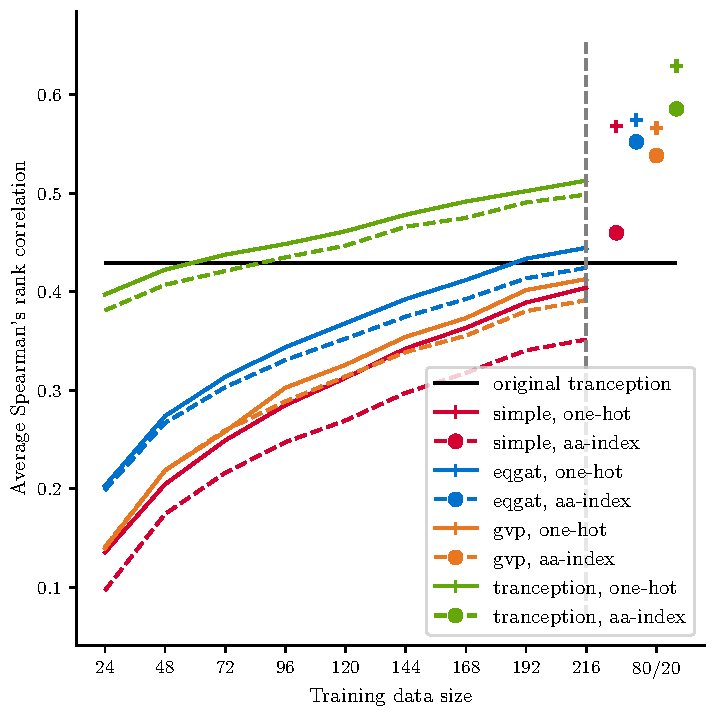
\includegraphics[width=0.45\textwidth]{masters-report/figures/spearmanr_all_square.pdf}\label{average-spearman-ridge-plot}} 
    \hspace{0.1in}
    \subfigure[We can improve the better than wildtype fitness prediction performance above the Tranception baseline (in black) across all regression models by training on as few as 144 data points.]{ 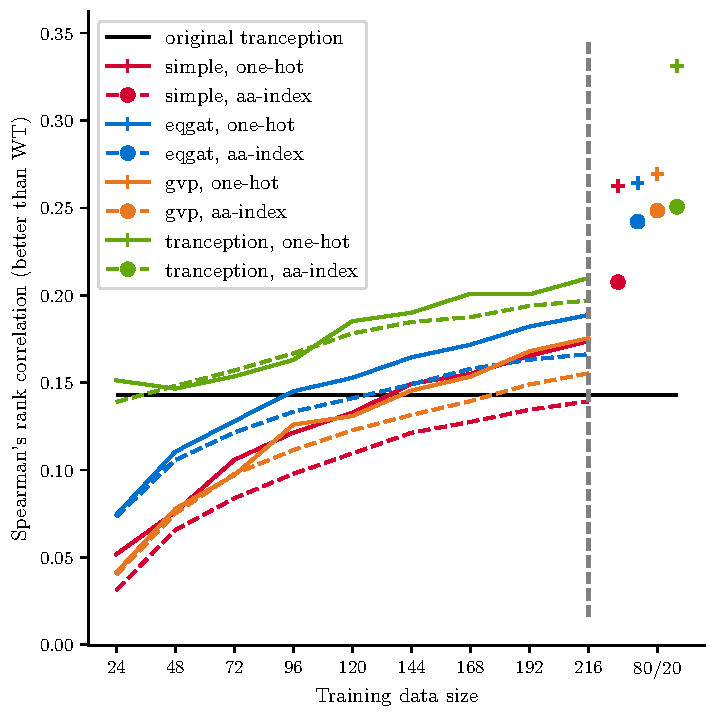
\includegraphics[width=0.45\textwidth]{masters-report/figures/better_than_WT_spearmanr_all_square.pdf}}
    \caption{Performance on mutations for four regression models using two types of embeddings. Statistics are aggregated across 49 DMS assays.}
    \label{one-hot-regression}
\end{figure}

I note from Figure \ref{average-spearman-ridge-plot} that with the exception of the EQGAT model, none of the other models exceed the unsupervised Tranception baseline within 216 training data points when I consider the Spearman rank correlation for the prediction of \textbf{all} fitness variants.

The augmented regressions with structure-based model scores can outperform the Tranception baseline on the better than wildtype Spearman correlation, but fail to do so within 216 samples for the overall Spearman correlation. This can be explained through the fact that, as we see in Table \ref{generation-results}, Tranception is far better than structure-based models at predicting the fitness of bad mutations. Hence, the baseline for overall fitness prediction is stronger. 



